\section{Sharpness of the reserve certificate}\label{sec:sharp}
Two statements delimit what Theorem~\ref{thm:anchor} and Theorem~\ref{thm:capacity} can be expected to give. The first shows that the regime hypothesis $x_*>\theta$ of the capacity law is not a technical artifact: below it, no amount of capacity helps. The second shows that in the opposite, high-renewal direction the anchored product is not merely an upper bound but is asymptotically exact.

\subsection{Capacity cannot compensate for an inadequate equilibrium}\label{sec:regime}
\begin{proposition}[Failure of the subcritical-reserve regime]\label{prop:regime}
Fix $\reff>m>0$ and $\theta\in(0,1)$ with $x_*=1-m/\reff<\theta$, and let
\[
 t_{\mathrm{cross}}
 =\frac1{\reff-m}\,\log\frac{m\theta}{\reff\theta-\reff+m}\in(0,\infty).
\]
For each integer $K$ let $H^K$ be the constant chain~\eqref{eq:healthy} started full, $H^K_0=K$, with threshold $h_{\min}=\lceil K\theta\rceil$. If $T>t_{\mathrm{cross}}$ then
\[
 \Prob(\tau_H\le T)\longrightarrow1\qquad(K\to\infty).
\]
Quantitatively, let $x$ solve $\dot x=\reff x(1-x)-mx$ with $x(0)=1$ and let $\varepsilon\in(0,\theta-x(T))$. Then
\begin{equation}\label{eq:fluid}
 \Prob(\tau_H\le T)\ \ge\
 1-\frac{4(\reff/4+m)\,T\,e^{2(\reff+m)T}}{K\varepsilon^2}.
\end{equation}
\end{proposition}

\begin{proof}
Put $X^K=H^K/K$. The chain is density dependent in the sense of \citet{kurtz1970}, and
\[
 X^K(t)=1+\int_0^t b(X^K(s))\,ds+\mathcal M_K(t),
 \qquad b(x)=\reff x(1-x)-mx,
\]
where $\mathcal M_K$ is a martingale whose jumps have size $1/K$ and whose predictable quadratic variation has rate $K^{-1}[\reff x(1-x)+mx]\le(\reff/4+m)/K$ on $[0,1]$. Doob's $L^2$ inequality gives
$\E\sup_{[0,T]}\mathcal M_K^2\le4(\reff/4+m)T/K$. On $[0,1]$ the drift $b$ is Lipschitz with constant $\reff+m$, so Gronwall's inequality yields
$\sup_{[0,T]}|X^K-x|\le e^{(\reff+m)T}\sup_{[0,T]}|\mathcal M_K|$, and Chebyshev's inequality gives~\eqref{eq:fluid} after substitution.

The deterministic equation is logistic with intrinsic rate $\reff-m$ and carrying level $x_*$, so from $x(0)=1>x_*$ its solution decreases to $x_*$ and is
\[
 x(t)=\frac{x_*}{1-(m/\reff)e^{-(\reff-m)t}}.
\]
Solving $x(t)=\theta$ gives exactly $t=t_{\mathrm{cross}}$, which is positive because $\theta<1$, and finite because $x_*<\theta$. Hence $x(T)<\theta$ for $T>t_{\mathrm{cross}}$, and $\varepsilon$ may be chosen as stated. On the event $\sup_{[0,T]}|X^K-x|\le\varepsilon$ we have $H^K_T<K\theta\le h_{\min}$, so $\tau_H\le T$. The complement has probability at most the displayed remainder.
\end{proof}

Proposition~\ref{prop:regime} is a statement about one constant healthy source, not an all-policy therapeutic exclusion; a policy that reduces $m$ changes $x_*$. Its force is comparative. Theorem~\ref{thm:capacity} makes failure exponentially small in $K$ when the equilibrium fraction $x_*$ exceeds the threshold fraction $\theta$, whereas here, with $x_*<\theta$, failure tends to one in $K$ for every horizon past a fixed crossing time. The sign of $x_*-\theta$, not the size of $K$, decides which regime the design is in, and the regime boundary is a property of rates rather than of scale. Adding units to a reserve whose equilibrium already sits below the functional threshold buys nothing.

\subsection{The anchored bound is exact at high renewal}\label{sec:highrenewal}
For a full reserve the natural anchor is the ceiling itself, $M=K$, and the buffer $d=K-h_{\min}$ is the number of units that must be lost in one excursion to fail.

\begin{proposition}[High-renewal limit and asymptotic sharpness]\label{prop:highrenewal}
Fix integers $1\le h_{\min}<K$, put $d=K-h_{\min}\ge1$, and fix $m,T>0$. For the constant chain~\eqref{eq:healthy} started at $H_0=K$:
\begin{enumerate}\itemsep2pt
\item[(i)] For every $\reff>0$ the top-anchor bound of Theorem~\ref{thm:anchor} with $M=K$ is exactly
\begin{equation}\label{eq:topexact}
 KmT\,P_{K-1}=\frac{(Km)^{d+1}T}{d!\,\reff^{\,d}}.
\end{equation}
\item[(ii)] Moreover
\begin{equation}\label{eq:limit}
 \lim_{\reff\to\infty}\reff^{\,d}\,\Prob_K(\tau_H\le T)
 =\frac{(Km)^{d+1}T}{d!}.
\end{equation}
\end{enumerate}
Hence the certificate~\eqref{eq:anchorbound} is sharp to leading order as $\reff\to\infty$, and the sufficient renewal requirement~\eqref{eq:renewalsizing} has the correct order in every parameter.
\end{proposition}

\begin{proof}
(i) With $M=K$ and $L=h_{\min}-1$, reindex the product in~\eqref{eq:scale} by $k=K-h$, which runs over $1,\ldots,d$:
\[
 P_{K-1}=\prod_{h=h_{\min}}^{K-1}\frac{Km}{\reff(K-h)}
 =\prod_{k=1}^{d}\frac{Km}{\reff k}=\frac{(Km)^d}{\reff^{\,d}\,d!}.
\]
Multiplying by $MmT=KmT$ gives~\eqref{eq:topexact}. In particular Theorem~\ref{thm:anchor} already yields the upper half of~\eqref{eq:limit},
\[
 \limsup_{\reff\to\infty}\reff^{\,d}\,\Prob_K(\tau_H\le T)\le\frac{(Km)^{d+1}T}{d!}.
\]

(ii) Write $q_r=q_K=P_{K-1}/D_K$ for the probability that an excursion leaving $K$ downward reaches $L$ before returning to $K$. Since $P_j$ is of order $\reff^{-(j-L)}$ for $j>L$ while $P_L=1$, we have $D_K\to1$ and
\begin{equation}\label{eq:qasym}
 q_r=\frac{(Km)^d}{d!\,\reff^{\,d}}\,(1+O(\reff^{-1})).
\end{equation}

Let $N_T$ be the number of downward departures from $K$ strictly before $\min(T,\tau_H)$. Its compensator is $Km\int_0^T\1_{\{H_s=K,\ s<\tau_H\}}ds$, so
\begin{equation}\label{eq:EN}
 \E N_T=Km\,\E\!\int_0^T\1_{\{H_s=K,\ s<\tau_H\}}\,ds.
\end{equation}
Failure is absorbing, so at most one excursion ever fails. By the strong Markov property at each departure and Wald's identity for the departure counting process,
\begin{equation}\label{eq:wald}
 \Prob(\hbox{some excursion begun before }T\hbox{ eventually fails})=q_r\,\E N_T .
\end{equation}
The event $\{\tau_H\le T\}$ differs from the event in~\eqref{eq:wald} only by excursions that begin before $T$ and fail after $T$. We control the two discrepancies in turn.

\emph{Excursion durations.} Let $D$ be the duration of an excursion from $K-1$ until it hits $\{L,K\}$. On the finitely many interior states $h\in\{h_{\min},\ldots,K-1\}$ the total jump rate satisfies
$\lambda_h+\mu_h\ge\reff h(K-h)/K\ge\reff c_*$ with
$c_*=\min_{h_{\min}\le h\le K-1}h(K-h)/K>0$, so every holding time is stochastically dominated by an exponential of rate $\reff c_*$. Moreover the upward one-step probability $\lambda_h/(\lambda_h+\mu_h)\to1$ uniformly on this finite set, so a block of at most $d$ consecutive jumps returns the chain to $K$ with probability bounded below uniformly in $\reff$ for $\reff$ large. The number of jumps before absorption is therefore dominated by a geometric number of such blocks, with $\reff$-independent mean, whence
\begin{equation}\label{eq:ED}
 \E D=O(\reff^{-1}).
\end{equation}

\emph{Occupation time at the ceiling.} The total time spent away from $K$ before $\min(T,\tau_H)$ is the sum over departures of the corresponding durations; by Wald and $\E N_T\le KmT$ it has expectation at most $KmT\,\E D=O(\reff^{-1})$. Time after absorption contributes at most $T\,\Prob(\tau_H\le T)=O(q_r)$. Hence the expectation in~\eqref{eq:EN} equals $T-O(\reff^{-1})-O(q_r)$ and
\begin{equation}\label{eq:ENasym}
 \E N_T=KmT+O(\reff^{-1})+O(q_r).
\end{equation}

\emph{Terminal correction.} Let $D_f$ be the excursion duration conditional on failure. Conditioning a killed birth--death chain on hitting $L$ before $K$ is a Doob $h$-transform by the harmonic function $p_\cdot$ of~\eqref{eq:ph}, which leaves holding rates unchanged and replaces the downward one-step probability at $h$ by
\[
 \frac{\mu_h\,p_{h-1}}{(\lambda_h+\mu_h)\,p_h}.
\]
Since $p_h\sim P_h$ and $P_{h-1}/P_h=\reff(K-h)/(Km)$, while
$\mu_h/(\lambda_h+\mu_h)=Km/[\reff(K-h)+Km]$, this probability tends to $1$ uniformly on the finite interior. Conditionally on failure the chain therefore makes $O(1)$ jumps at rates at least $\reff c_*$, so $\E D_f=O(\reff^{-1})$ by the same block argument. Using the departure intensity bound and the strong Markov property, the expected number of excursions that begin before $T$ and fail after $T$ is at most
\[
 Km\,q_r\int_0^T\Prob(D_f>T-s)\,ds\ \le\ Km\,q_r\,\E D_f=O(q_r\reff^{-1}).
\]

Combining this with~\eqref{eq:wald}, \eqref{eq:ENasym} and~\eqref{eq:qasym},
\[
 \Prob(\tau_H\le T)=q_r\,\E N_T+O(q_r\reff^{-1})
 =\frac{(Km)^{d+1}T}{d!\,\reff^{\,d}}\bigl(1+O(\reff^{-1})\bigr),
\]
which is~\eqref{eq:limit}.
\end{proof}

\begin{figure}[tb]
 \centering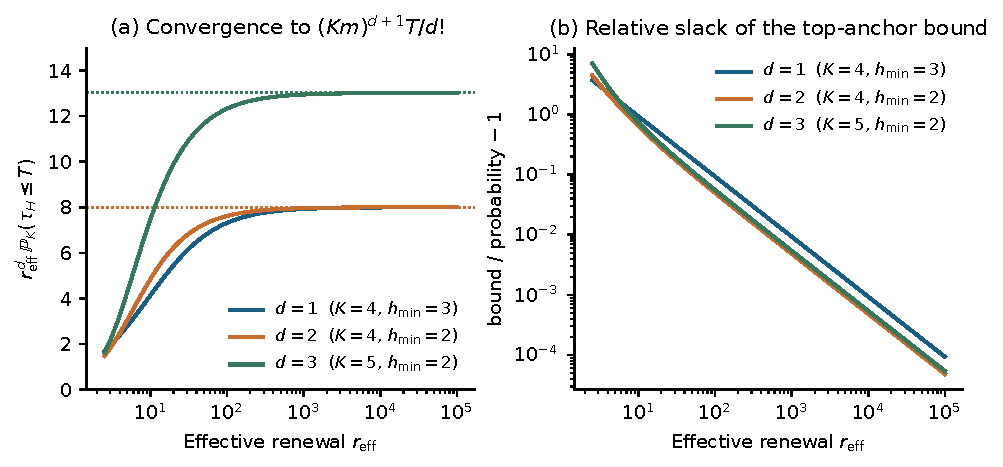
\includegraphics[width=.96\linewidth]{figures/high_renewal.pdf}
 \caption{Proposition~\ref{prop:highrenewal} against exact computation. (a) $\reff^{\,d}\Prob_K(\tau_H\le T)$ for the constant chain started full, at $m=1/2$ and $T=2$, obtained from the killed Kolmogorov equation; dotted lines mark the predicted constants $(Km)^{d+1}T/d!$, which equal $8$, $8$ and $625/48$ respectively. (b) Relative slack of the top-anchor bound~\eqref{eq:topexact}, which decays like $1/\reff$. Because the probabilities reach $10^{-15}$ and below, these curves were evaluated at $60$ decimal digits; in double precision the subtraction $1-\sum_j p_{Kj}(T)$ loses all significant figures and can appear to violate the proved bound. The bound exceeds the exact probability at every plotted point.}\label{fig:highrenewal}
\end{figure}

\begin{remark}[Depleted preparations have a different exponent]\label{rem:depleted}
The exponent in~\eqref{eq:limit} is a property of a \emph{full} reserve. If instead $h_{\min}\le h_0<K$, the initial scale-function term of Corollary~\ref{cor:initial} is itself of order $\reff^{-(h_0-h_{\min}+1)}$, so the failure probability is of order $\reff^{-\min\{d,\;h_0-h_{\min}+1\}}$. One may not transfer the fully filled exponent to a depleted preparation: a reserve that begins one unit above the threshold gains only a single power of renewal, however large the buffer $d$ is.
\end{remark}

\begin{remark}[What is not claimed]\label{rem:notclaimed}
Proposition~\ref{prop:highrenewal} is a homogeneous statement with fixed $K,m,T$. It does not license replacing $m$ by a time-varying $m(t)$, interchanging the limit with an arbitrary schedule, or deriving a Jensen-type optimal scheduling law. A time-varying version would need inhomogeneous conditional-excursion estimates and an $o(\reff^{-d})$ remainder that is uniform over rate profiles; renewal-dependent oscillations are a concrete obstruction. We therefore leave the time-varying coefficient open and do not use it anywhere below.
\end{remark}
